\section{Essential Array Questions: An Introduction}
\label{sec:EssentialArrayQuestions}

Arrays are among the most fundamental data structures in computer science, serving as the backbone for numerous algorithms and problem-solving strategies. Mastering essential array-related problems is crucial for excelling in technical interviews and understanding core algorithmic concepts. These problems often explore key topics such as subarray manipulation, prefix sums, hash keying, and sliding windows. 

This section introduces a curated collection of essential array problems designed to cover a wide range of techniques and scenarios. Each problem emphasizes different aspects of array manipulation, optimization strategies, and algorithm design, ensuring comprehensive preparation. The following problems are presented with detailed explanations, algorithmic approaches, and Python implementations to solidify your understanding and equip you for success.

\problemsection{Best Time to Buy and Sell Stock}
\label{problem:Best_Time_to_Buy_and_Sell_Stock}

The "Best Time to Buy and Sell Stock" problem is a common interview question that assesses a candidate's ability to work with arrays and apply dynamic programming concepts. The problem requires finding the optimal buy and sell times to maximize profit from a series of daily stock prices.

\section*{Problem Statement}
You are given an array \texttt{prices}, where \texttt{prices[i]} is the price of a given stock on the \(i\)th day. Your goal is to determine the maximum profit obtainable by buying on one day and selling on a later day. If no profit can be made, return 0.



\begin{figure}[h]
  \centering
  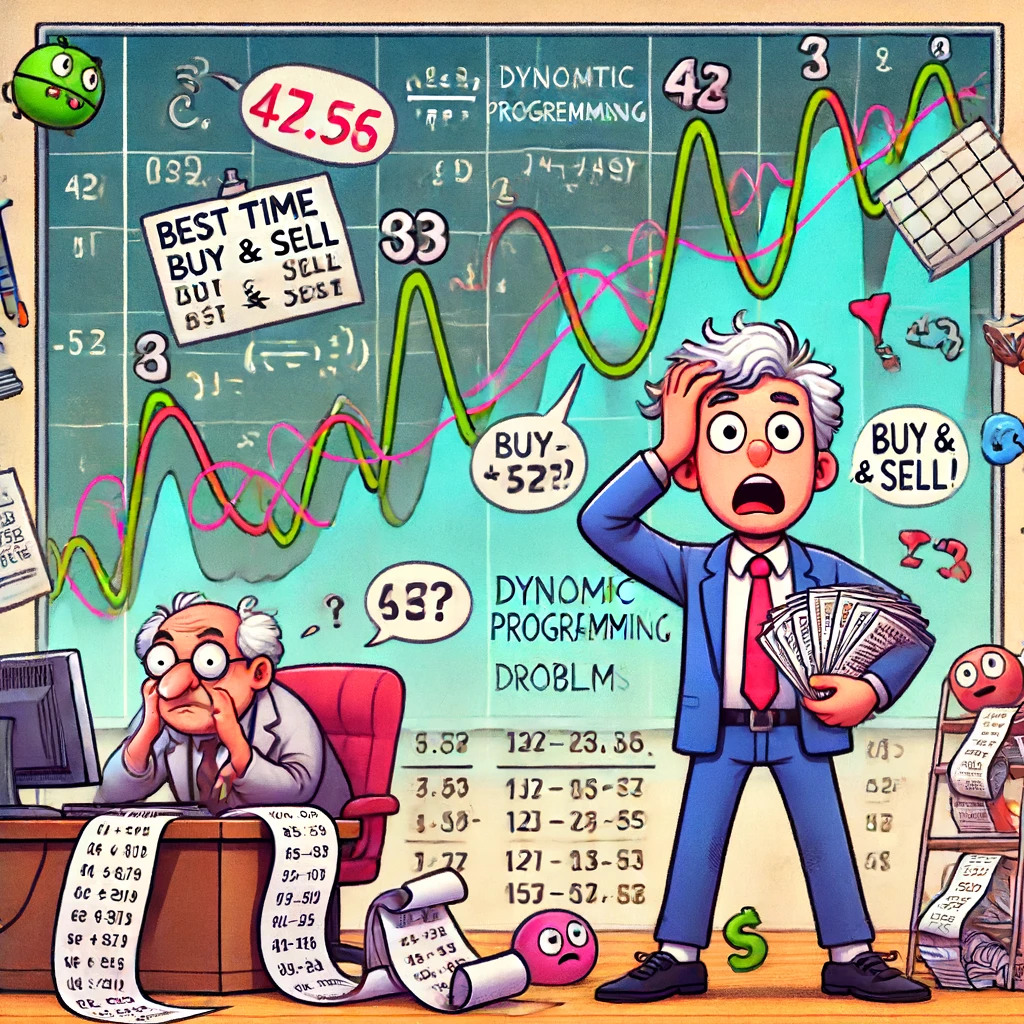
\includegraphics[width=\mywidth]{figs/stock}  % Ensure the correct file path and extension
  \caption{Best Time to Buy and Sell Stock.}
\end{figure}

\textbf{Input:} An array \texttt{prices}, with \texttt{prices[i]} representing the stock price on the \(i\)th day.

\textbf{Output:} The maximum profit that can be achieved.

\textbf{Example 1:}
\begin{verbatim}
    Input: prices = [7,1,5,3,6,4]
    Output: 5
    Explanation: Buy on day 2 (price = 1) and sell on day 5 (price = 6), 
    profit = 6 - 1 = 5.
\end{verbatim}

\textbf{Example 2:}
\begin{verbatim}
    Input: prices = [7,6,4,3,1]
    Output: 0
    Explanation: No transaction can yield a profit, hence the max profit = 0.
\end{verbatim}

\section*{Algorithmic Approach}
The common approach to solving this problem is to use a single pass. Iterate through the \texttt{prices} array while tracking the minimum price encountered so far. For each price, calculate the profit if the stock were sold at that price, updating the maximum profit as necessary.

\section*{Complexities}
\begin{itemize}
    \item \textbf{Time Complexity:} \(O(n)\), where \(n\) is the number of days, since it requires a single pass through the array.
    \item \textbf{Space Complexity:} \(O(1)\), as only a constant amount of extra space is needed for variables such as \texttt{min\_price} and \texttt{max\_profit}.
\end{itemize}

\section*{Python Implementation}
The Python implementation uses the above algorithm to find the maximum profit with a single pass through the stock prices:

\begin{fullwidth}
\begin{lstlisting}[language=Python]
class Solution:
    def maxProfit(self, prices: List[int]) -> int:
        min_price = float('inf')  # Initialize to positive infinity
        max_profit = 0
        
        # Loop through all stock prices
        for price in prices:
            # Updating the minimum price seen so far
            if price < min_price:
                min_price = price
            # Computing potential profit and update max profit
            elif price - min_price > max_profit:
                max_profit = price - min_price
        return max_profit
\end{lstlisting}

\end{fullwidth}

This approach initializes the minimum price to infinity and the maximum profit to 0 and iterates over the \texttt{prices} array. For each stock price, it checks if the price is lower than the current minimum price. If it is, the minimum price is updated. Otherwise, it calculates the profit one would get if one sold at the current price and updates the maximum profit if the current profit is larger. After iterating through all the prices, the maximum profit is returned.

\section*{Why This Approach}
This approach is chosen for its efficiency in both time and space. It navigates the array only once, ensuring a linear time complexity, which is optimal in this case because you have to examine each price at least once to determine the profit.

\section*{Alternative Approaches}
Alternative methods might use more complex data structures, such as segment trees, to perform many queries on the range of days. However, this is overkill for the given problem and would not improve the best-case time complexity.

\section*{Similar Problems to This One}
Similar problems include variations that allow for multiple transactions, incorporate a cooldown period between sales, or limit the number of transactions.

\section*{Things to Keep in Mind and Tricks}
One trick for problems like this is to consider the running difference between the current and minimum prices as the "current profit" and to update the maximum profit if a higher current profit is found.

\section*{Corner and Special Cases to Test When Writing the Code}
Test cases should include:
- Increasing and decreasing prices, ensuring profit is calculated correctly or confirmed as zero.
- Large input arrays to verify performance.
- Edge cases with the minimum input size (e.g., an array of just one price).

\section*{Explanation of Sliding Window Concept}
In this problem, the sliding window is not explicitly represented by two pointers, but the concept is similar. The window dynamically adjusts as we iterate through the \texttt{prices} array, always keeping track of the lowest buying price and the highest potential selling price after that buying day. This ensures that each price is considered only once, resulting in a linear time complexity of \(O(n)\)\sidenote{Linear time complexity}.